\documentclass{article}
\usepackage{setspace}
\usepackage[text={6.5in,8.5in},centering]{geometry}
\geometry{verbose,a4paper,tmargin=2.4cm,bmargin=2.4cm,lmargin=2.4cm,rmargin=2.4cm}
\usepackage{graphicx,amsmath,cases,multirow,appendix,graphicx,xcolor}

\setlength\parindent{0pt}

\newcommand{\note}[1]{\colorbox{gray!30}{#1}}
\newcommand{\ind}{\-\hspace{1cm}}

\begin{document}

\noindent\makebox[\textwidth][c]{\Large\bfseries Lecture 8 -- 1-D Stability Analysis}
\rule[0.5ex]{\linewidth}{1pt}
\textbf{Future:}
Dynamics \& Stability \& Species-coexistence\\
\ind \ind - 1-sp. models (limit-cycles \& chaos)\\
\ind \ind - 2 spp. models (linear \& non-linear models)\\
\ind \ind - 3 spp. models (indirect effects)\\
\ind \ind - $n$ spp. models\\
\ind \emph{ = unstructured models} (but methods apply to structured models too!)

\rule[0.5ex]{\linewidth}{1pt}

\textbf{Concepts:}\\
\ind Stable point-equilibrium vs. Stable limit cycles vs. Deterministic chaos\\
\ind Time-delays / Response-lags \& Over- and under-compensation\\
\ind Formal local stability analysis

\rule[0.5ex]{\linewidth}{1pt}

\textbf{Quick review:} \note{Overlay on same three graphs}\\
Discrete-time difference equation: $N_{t+1}=F(N_t)$\\
\begin{equation*}
	F(N_t)=N_t + r_d N_t \to \; \text{geometric growth}
\end{equation*}

\begin{center}
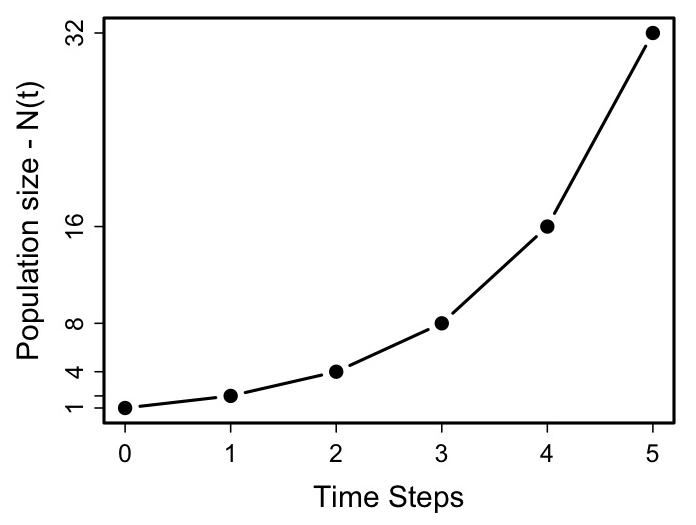
\includegraphics[width=5cm]{figs/a.png}
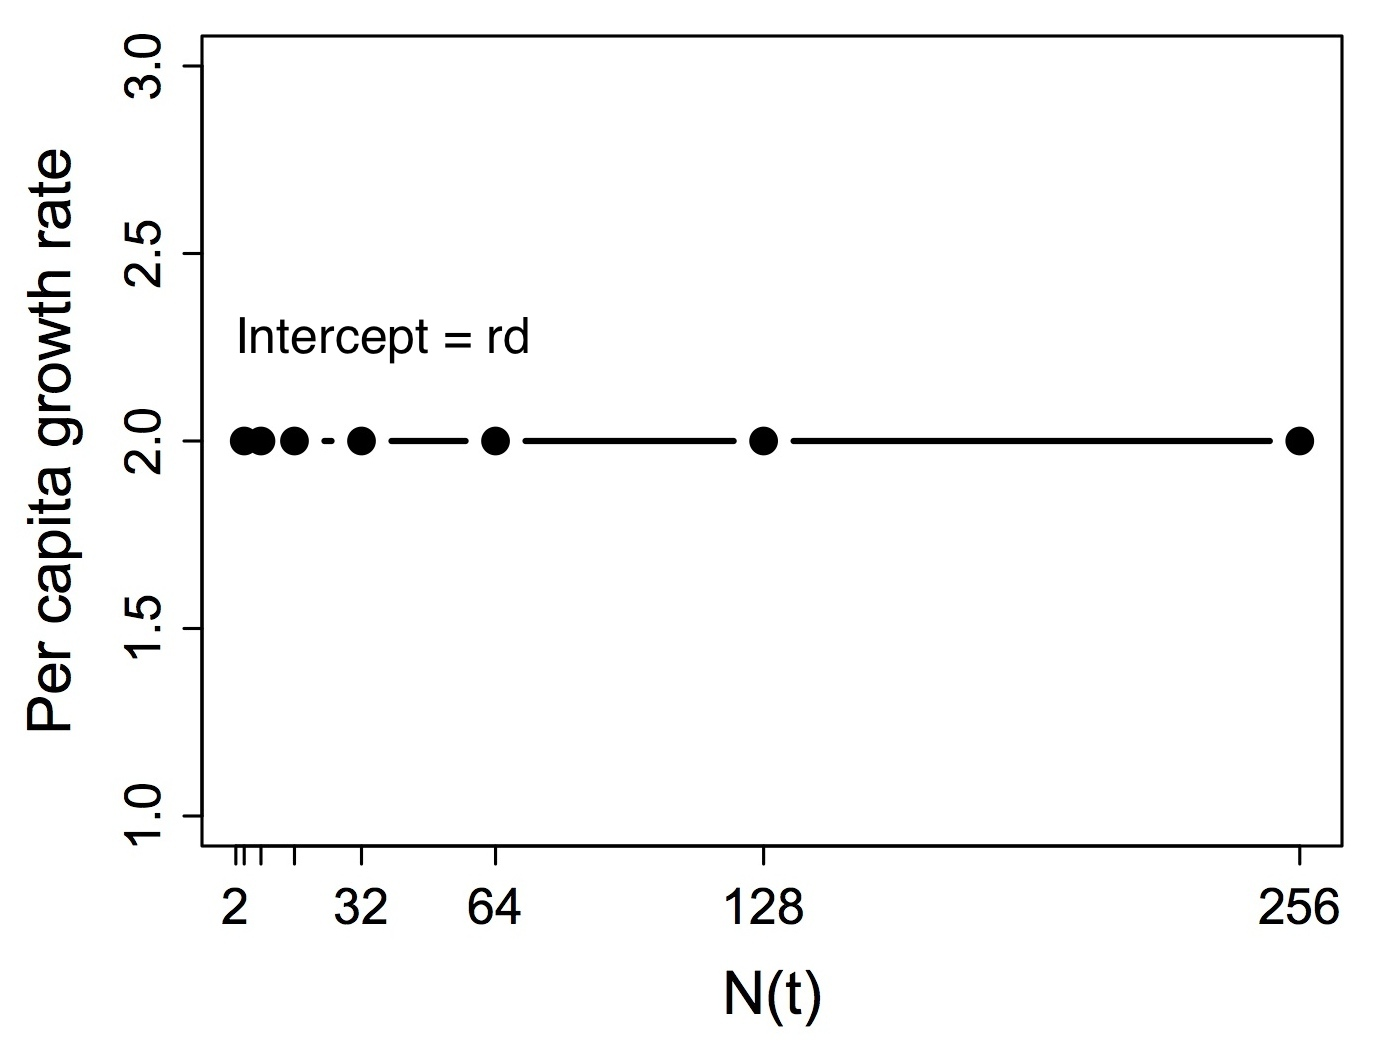
\includegraphics[width=5cm]{figs/b.jpg}
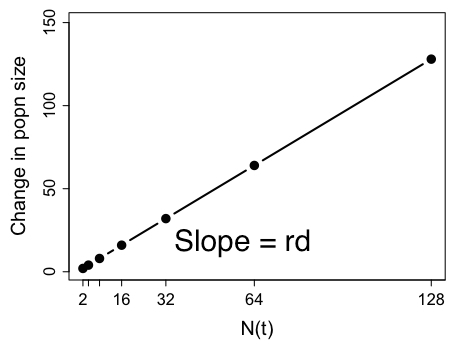
\includegraphics[width=5cm]{figs/c.jpg}
\end{center}

\begin{equation*}
	F(N_t)=N_t + r_d N_t \left(1-\frac{N_t}{K}\right) \to \; \text{discrete logistic growth}
\end{equation*}
\begin{center}
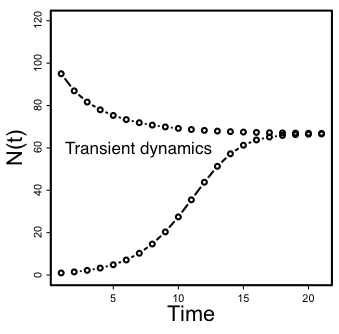
\includegraphics[width=4.5cm]{figs/d.png}
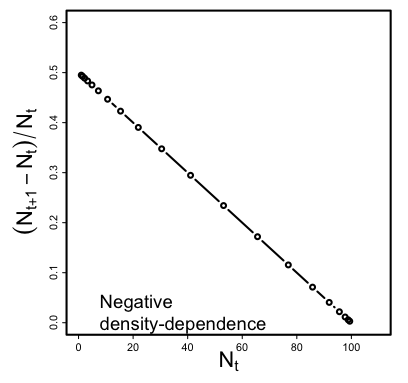
\includegraphics[width=4.5cm]{figs/e.png}
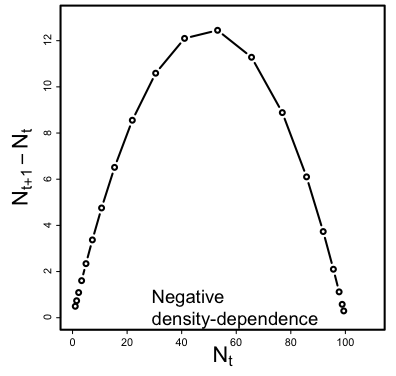
\includegraphics[width=4.5cm]{figs/f.png}
\end{center}

Notice \textbf{transient} versus \textbf{steady-state/equilibrial} dynamics.

\rule[0.5ex]{\linewidth}{1pt}


\textbf{R-code exercise - Increasing $r_d$}\\
\note{First walk through \emph{Class-Ex-Chaos.R}.}  \\
\note{Let class experiment with $r_d$ (assuming $K=10$)} (look at \emph{out} vector after transients)

\begin{table*}[h]
\centering
\begin{tabular}{cc}
$\mathbf{r_d}$ & \textbf{Number of different popn sizes} \\ 
\hline
 $<2$ & monotonic dampening \& damped oscillations \\ 
2 &  2-point \\ 
2.449 & 4-point \\ 
2.544 & 8-point \\ 
2.564 &  16-point\\ 
2.5687 & 32-point \\ 
$> 2.7$ & deterministic chaos \\ 
 \hline
\end{tabular} 
\end{table*}

\note{Let class experiment with $r_d<2.7$ at different $N_0$.}\\
Conclusion:\\
 \ind $\to$ Period doubling bifurcations\\
\ind \ind $\to$ \textbf{Stable limit cycles} (stable attractor orbits independent of initial conditions)

\textbf{Deterministic chaos-} Sensitivity to initial conditions\\
\note{Experiment with $r_d > 2.7$ at different $N_0$} \\
\ind (look at \emph{out} vector with $N_0=0.0100...001$, up to computer precision $<10^{-18}$)

\begin{table*}[h]
\centering
\begin{tabular}{ll}
$\mathbf{N_0}$ & $\mathbf{N_{t=2000}}\;\; (r_d-3)$ \\ 
\hline
0.01 & 13.26...\\
0.011 & 12.46... \\
0.01001 & 0.37... \\
$0.01 + 1 \cdot 10^{-10} $ & 8.05...\\
$ 0.01 + 1 \cdot 10^{-18} $ & 2.25...\\
\hline
\end{tabular} 
\end{table*}

$\to$ Not stochastic!  Rather, deterministic!

\rule[0.5ex]{\linewidth}{1pt}

\textbf{Bifurcation plot} - Popn points as function of focal parameter.

\ind \note{Work through \emph{peaks} function}\\
\ind \note{Run code and explain plot}\\
\ind \note{Add to table $r_d=2.83 \to$ 3-point cycle.}

\rule[0.5ex]{\linewidth}{1pt}

\textbf{Lyapunov exponent} - $\lambda$ (not popn growth rate!)\\
\ind Measure of sensitivity to initial conditions.\\
\begin{equation*}
	\vert \Delta_t \vert = \vert \Delta_0 \vert \cdot  e^{t \lambda}
\end{equation*}
\ind \ind where $N_0 + \Delta_0$ is some small addition to $N_0$.\\
That is,
\begin{equation*}
	\vert \Delta_t \vert = \vert \; F(N_0 + \Delta_0)_t - F(N_0)_t \; \vert
\end{equation*}
Rearrange to:
\begin{equation*}
	\lambda = \frac{log\left(\frac{\vert \Delta_t \vert}{\vert \Delta_0 \vert} \right)}{t}
\end{equation*}

\begin{center}
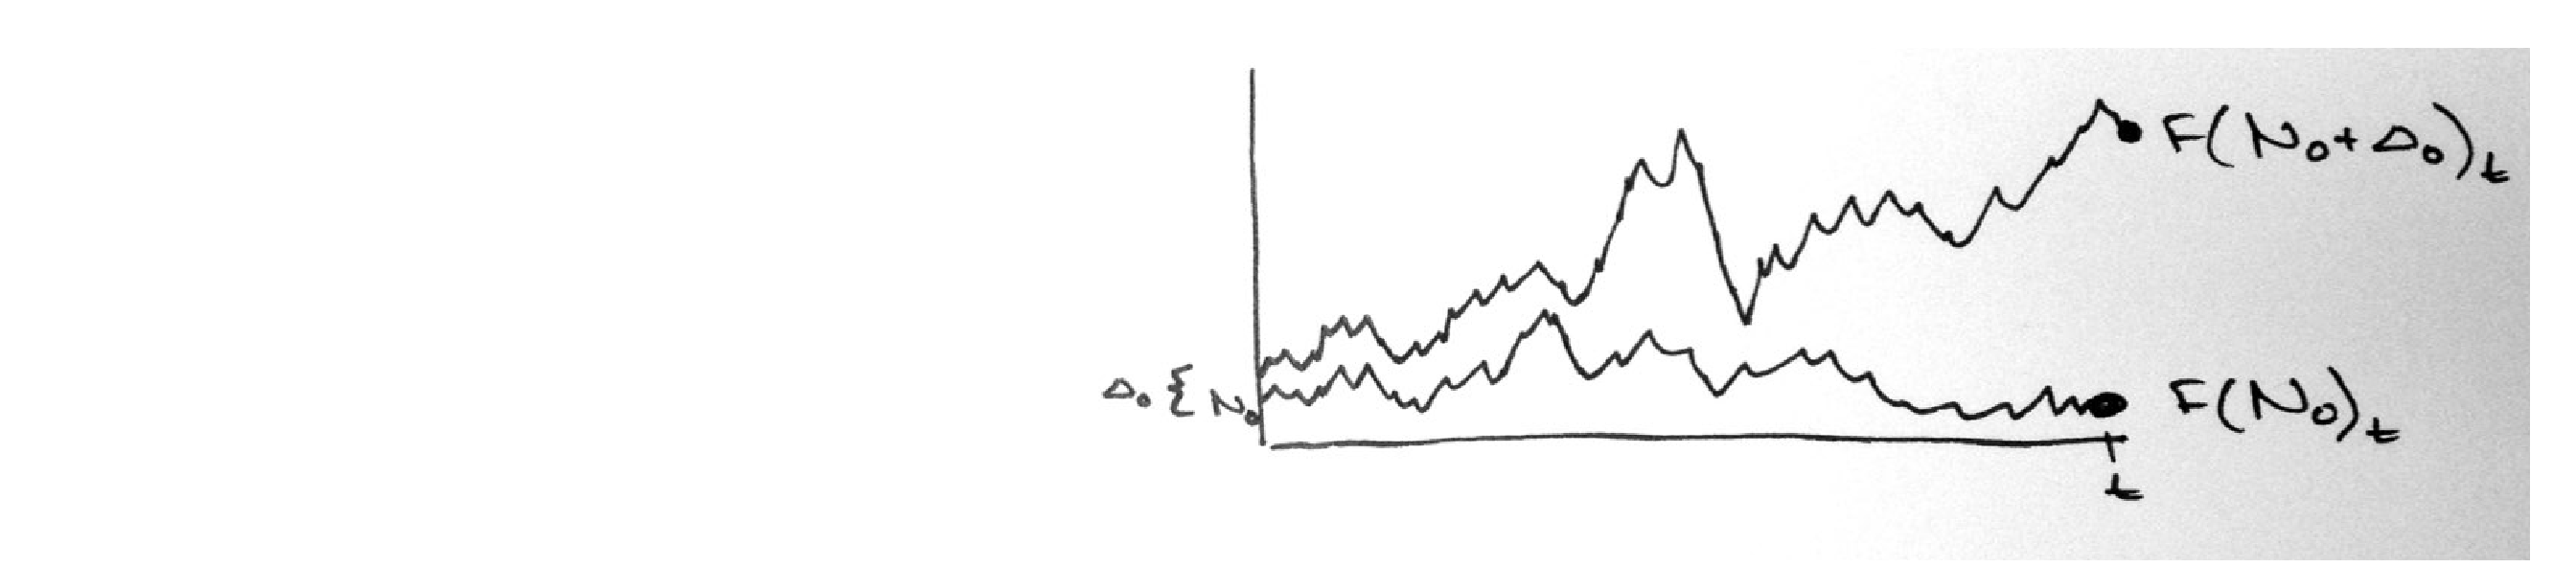
\includegraphics[width=8cm]{figs/Lyapunov.pdf}
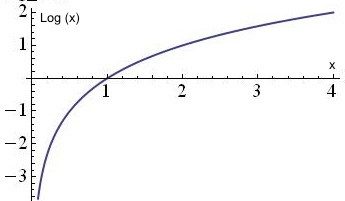
\includegraphics[width=4.5cm]{figs/log.jpg}
\end{center}

Thus,
\ind If $\lambda < 0,  \to $ convergence $\to$ same dynamics $\to$ point equilibrium or limit cycle\\
\ind \ind If $\lambda > 0,  \to $ diverging dynamics $\to$ chaos

\begin{center}
\note{Show in Keynote w/ animation}
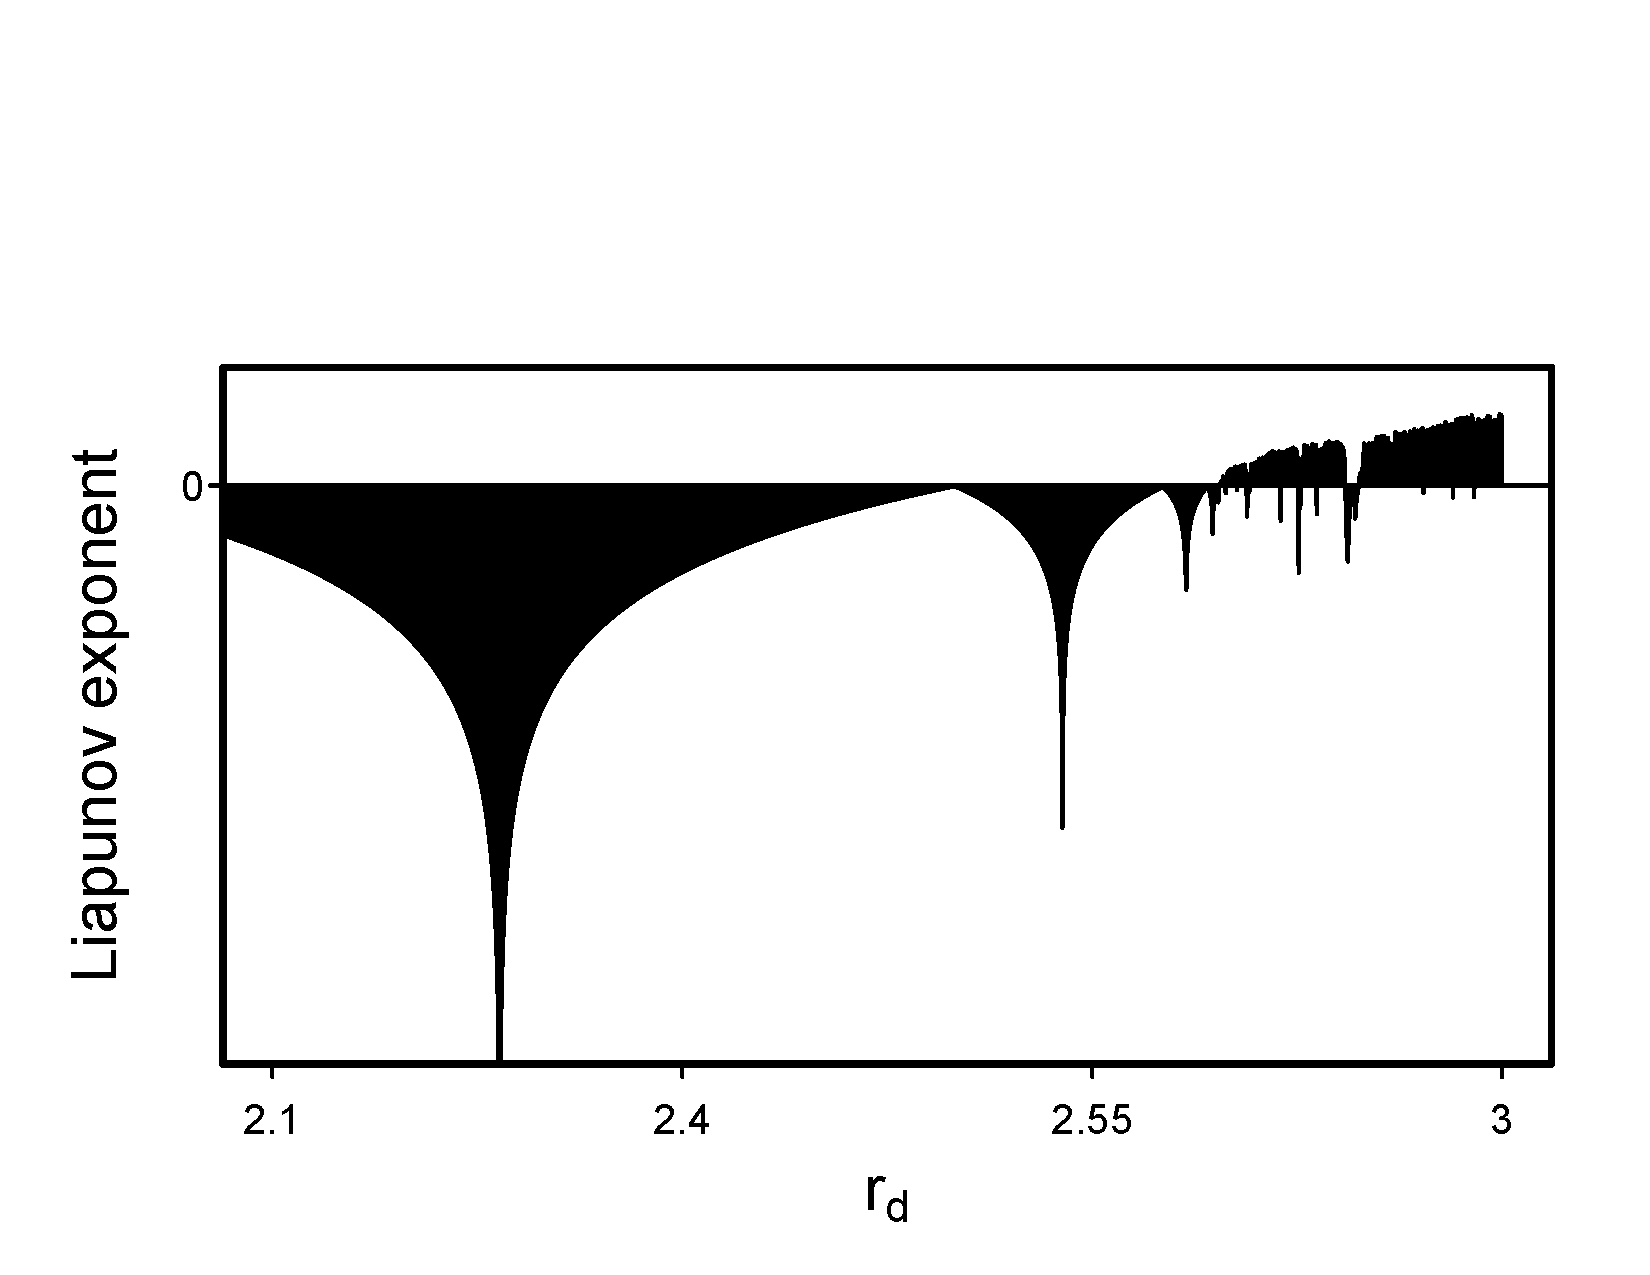
\includegraphics[width=6cm]{figs/Lyapunov2.pdf}
\end{center}

\rule[0.5ex]{\linewidth}{1pt}
\pagebreak

\textbf{Mechanism:}\\
$N_{t+1} = F(N_t)$ contains implicit time-lag of 1 unit time\\
\ind $\to$ over- and under-compensation (like lagged thermostat)

\textbf{Contrast to continuous-time model} (differential eqn)\\
\begin{equation*}
	\frac{dN}{dt}=rN\left(1-\frac{N}{K}\right)
\end{equation*}
\note{Work through and run last section of R-code.}

\textbf{Contrast to delay-differential model}
\begin{equation*}
	\frac{dN}{dt}=rN_{t-\tau}\left(1-\frac{N_{t-\tau}}{K}\right)
\end{equation*}
Note: For simple delay model, only 2-point limit cycle.  \\
\ind  Either need more delays on variables or $>2$ species to get more complex dynamics.

\rule[0.5ex]{\linewidth}{1pt}

\note{Switch to pdf of Keynote presentation of examples}\\
\ind - \emph{Daphnia} example from Case\\
\ind \ind \note{Class Q:} Why is Case's use as an example of period-doubling wrong!?!\\
\ind \ind \note{A:} \emph{Daphnia} exhibit continuous reproduction (w/ lag)! (see slide)\\
\ind - Flour beetles\\
\ind - Hassel \& May insect dynamics\\
\ind - Other examples: Herring, Salmon, Cicadas\\

\rule[0.5ex]{\linewidth}{1pt}

\textbf{Ricker Plots} \note{Class exercise - handout}\\
To develop more intuitive notion of (implicit) time-lag and over- \& under-compensation.\\
Note that time-lag is also implicit in interspecific species interactions.\\
Assume discrete-time logistic...

\begin{center}
	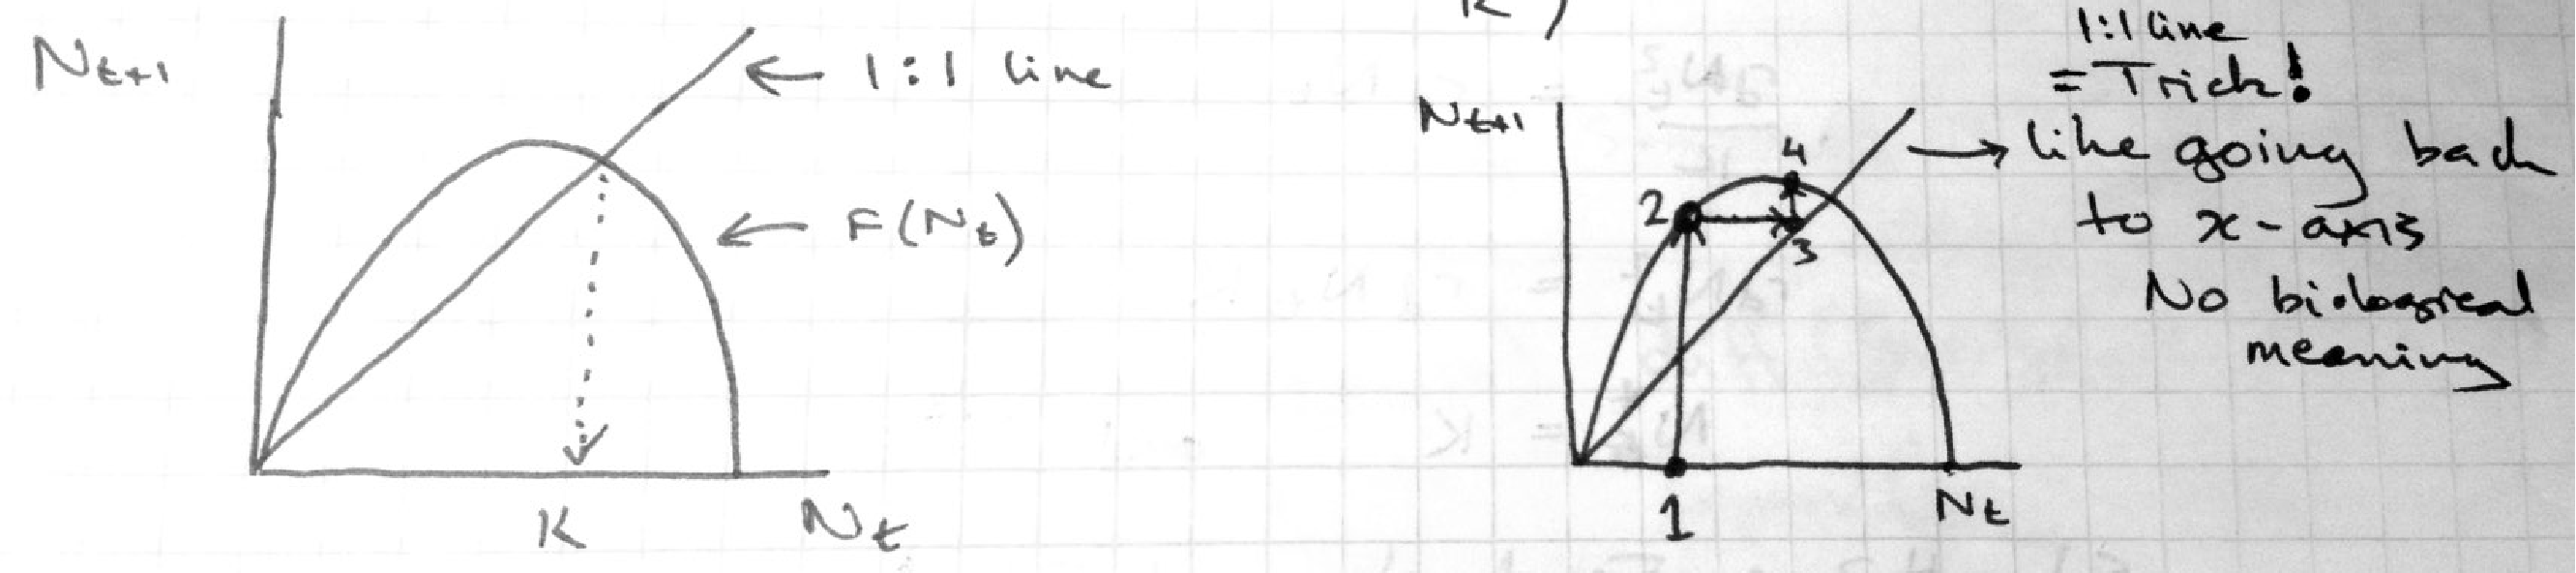
\includegraphics[width=12cm]{figs/RickerCurve.pdf}
\end{center}

\note{Class Q:} Can you predict dynamics from shape of plot?\\

\rule[0.5ex]{\linewidth}{1pt}
\end{document}